% -*- compile-command: "make HOCKING-PeakSeg-functional-pruning-slides.pdf" -*-
\documentclass{beamer}
\usepackage{tikz}
\usepackage[all]{xy}
\usepackage{amsmath,amssymb}
\usepackage{hyperref}
\usepackage{graphicx}
\usepackage{algorithmic}

\DeclareMathOperator*{\argmin}{arg\,min}
\DeclareMathOperator*{\Lik}{Lik}
\DeclareMathOperator*{\PoissonLoss}{PoissonLoss}
\DeclareMathOperator*{\Peaks}{Peaks}
\DeclareMathOperator*{\Segments}{Segments}
\DeclareMathOperator*{\argmax}{arg\,max}
\DeclareMathOperator*{\maximize}{maximize}
\DeclareMathOperator*{\minimize}{minimize}
\newcommand{\sign}{\operatorname{sign}}
\newcommand{\RR}{\mathbb R}
\newcommand{\ZZ}{\mathbb Z}
\newcommand{\NN}{\mathbb N}

% Set transparency of non-highlighted sections in the table of
% contents slide.
\setbeamertemplate{section in toc shaded}[default][100]
\AtBeginSection[]
{
  \setbeamercolor{section in toc}{fg=red} 
  \setbeamercolor{section in toc shaded}{fg=black} 
  \begin{frame}
    \tableofcontents[currentsection]
  \end{frame}
}

\begin{document}

\title{A linear time algorithm for constrained 
optimal segmentation}

\author{
  Toby Dylan Hocking\\
  toby.hocking@mail.mcgill.ca\\
  joint work with Guillem Rigaill, Paul Fearnhead, 
  Guillaume Bourque}

\date{11 Aug 2016}

\maketitle

\section{Problem: optimizing ChIP-seq peak detection}

\begin{frame}
  \frametitle{Chromatin immunoprecipitation sequencing (ChIP-seq)}
  Analysis of DNA-protein interactions.

  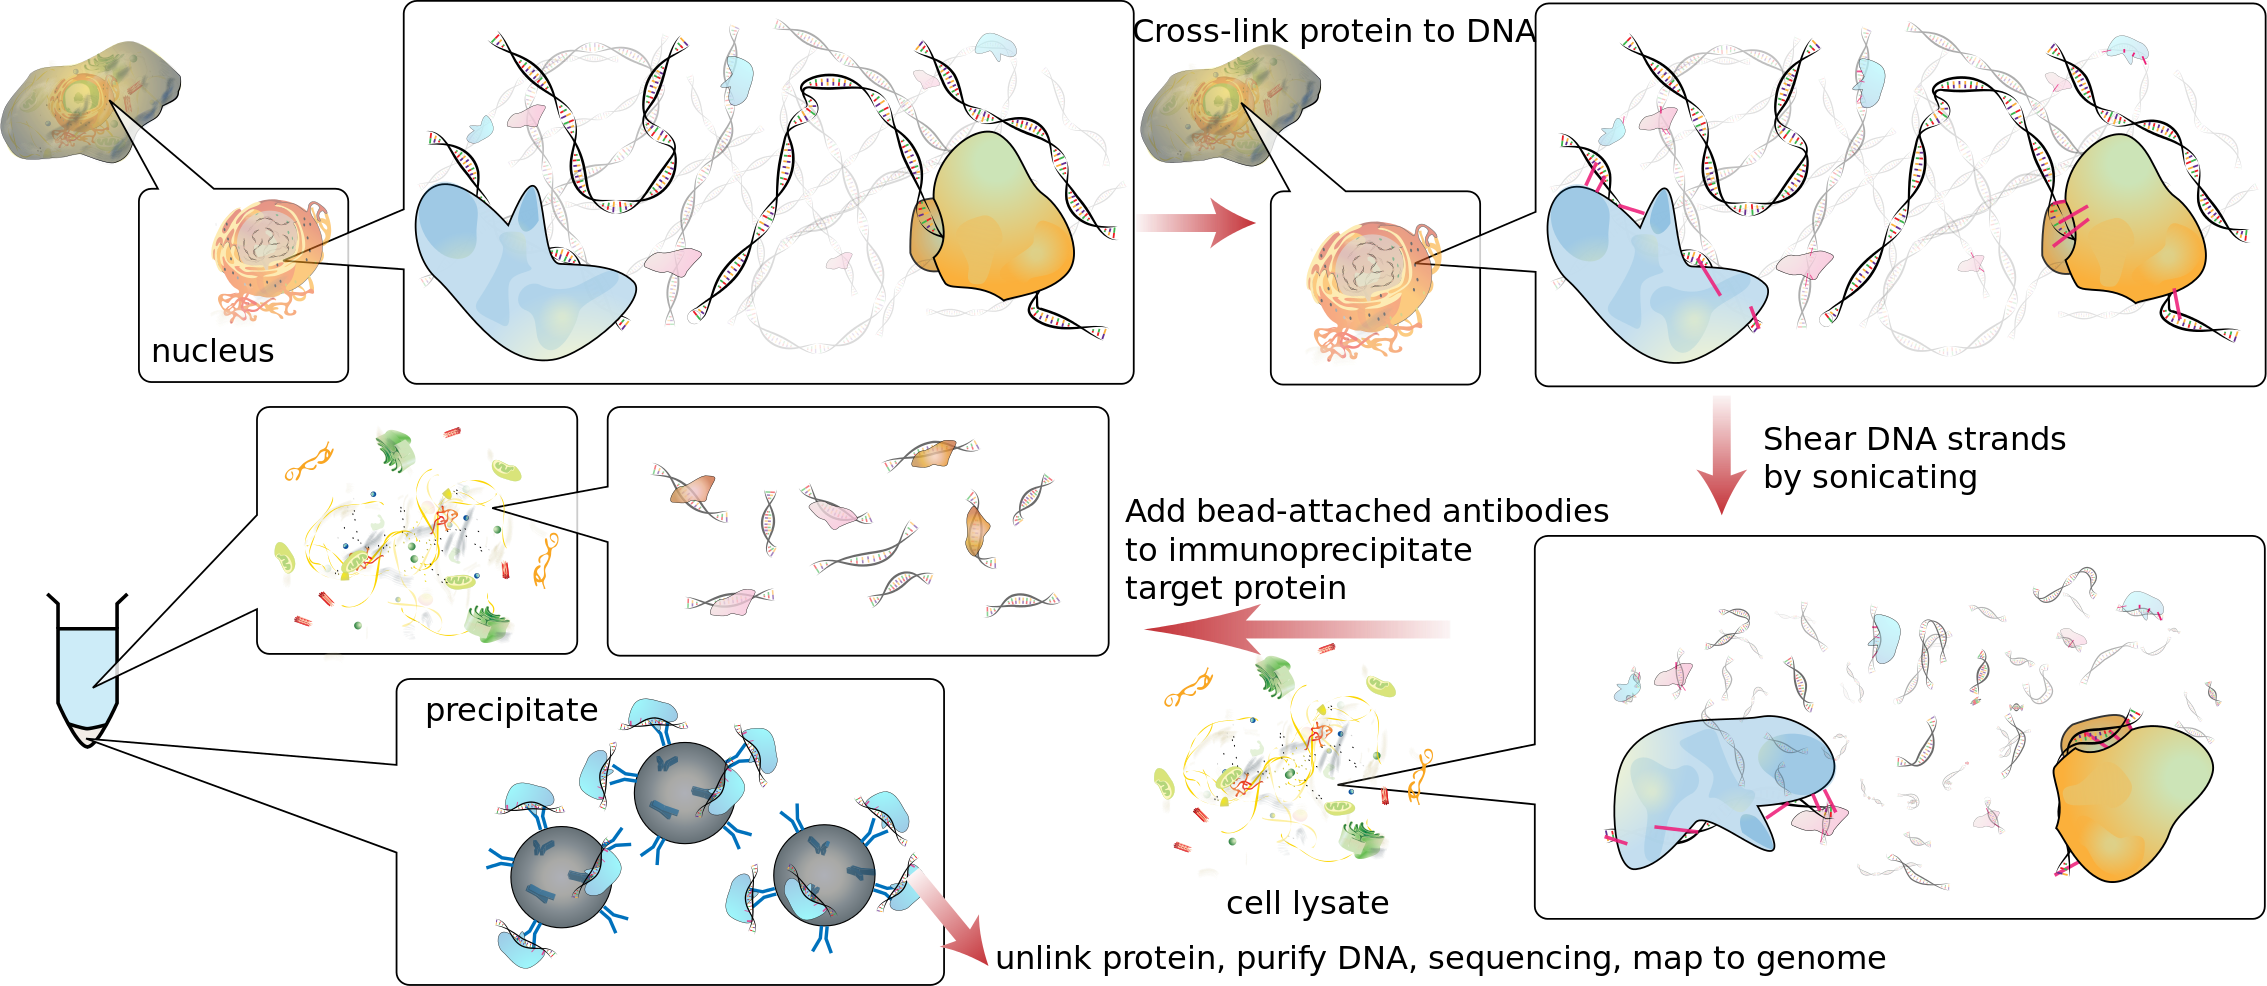
\includegraphics[width=\textwidth]{Chromatin_immunoprecipitation_sequencing_wide.png}

  Source: ``ChIP-sequencing,'' Wikipedia.
\end{frame}

\begin{frame}
  \frametitle{Problem: find peaks in each of several samples}
  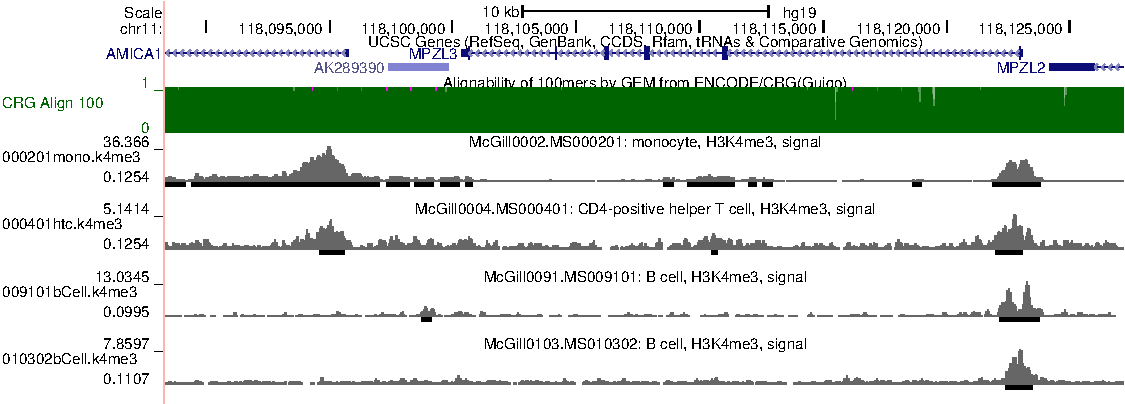
\includegraphics[width=\textwidth]{screenshot-ucsc-edited}

  Grey profiles are normalized aligned read count signals.

  Black bars are ``peaks'' called by MACS2 (Zhang et al, 2008):
  \begin{itemize}
  \item many false positives.
  \item overlapping peaks have different start/end positions.
  \end{itemize}
\end{frame}

\begin{frame}
  \frametitle{Previous work in genomic peak detection}
  \begin{itemize}
  \item Model-based analysis of ChIP-Seq (MACS), Zhang et al, 2008.
  \item SICER, Zang et al, 2009.
  \item HOMER, Heinz et al, 2010.
  \item CCAT, Xu et al, 2010.
  \item RSEG, Song et al, 2011.
  \item Triform, Kornacker et al, 2012.
  \item Histone modifications in cancer (HMCan), Ashoor et al, 2013.
  \item PeakSeg, Hocking, Rigaill, Bourque, ICML 2015.
  \item PeakSegJoint Hocking and Bourque, arXiv:1506.01286.
  \item ... dozens of others.
  \end{itemize}
  Two big questions: how to choose the best...
  \begin{itemize}
  \item ...algorithm? (testing)
  \item ...parameters? (training)
  \end{itemize}
\end{frame}

\begin{frame}[fragile]
  \frametitle{How to choose parameters of unsupervised peak
    detectors?}
\scriptsize
19 parameters for Model-based analysis of ChIP-Seq (MACS), Zhang et al, 2008.
\begin{verbatim}
  [-g GSIZE]
  [-s TSIZE] [--bw BW] [-m MFOLD MFOLD] [--fix-bimodal]
  [--nomodel] [--extsize EXTSIZE | --shiftsize SHIFTSIZE]
  [-q QVALUE | -p PVALUE | -F FOLDENRICHMENT] [--to-large]
  [--down-sample] [--seed SEED] [--nolambda]
  [--slocal SMALLLOCAL] [--llocal LARGELOCAL]
  [--shift-control] [--half-ext] [--broad]
  [--broad-cutoff BROADCUTOFF] [--call-summits]
\end{verbatim}
10 parameters for Histone modifications in cancer (HMCan),
Ashoor et al, 2013.
\begin{verbatim}
minLength 145
medLength 150
maxLength 155
smallBinLength 50
largeBinLength 100000
pvalueThreshold 0.01
mergeDistance 200
iterationThreshold 5
finalThreshold 0
maxIter 20
\end{verbatim}
\end{frame}

\begin{frame}
  \frametitle{Which macs parameter is better for these data?}
  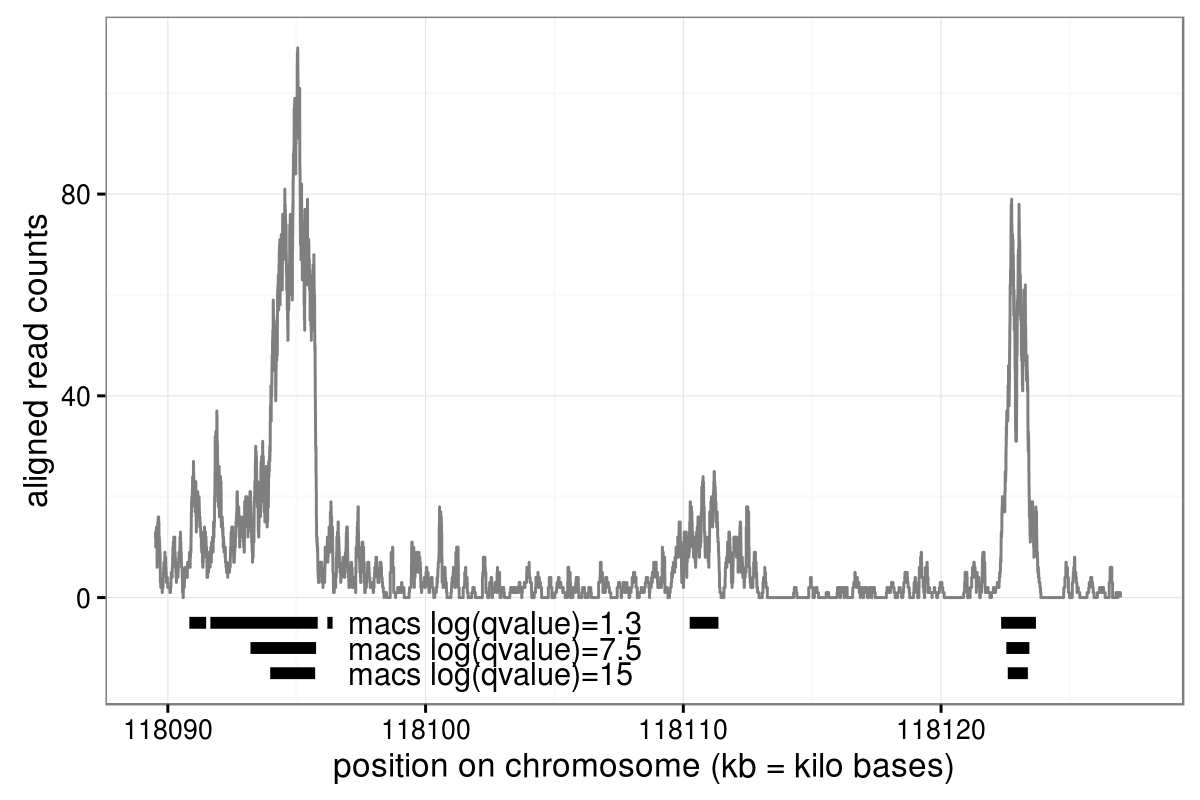
\includegraphics[width=1\textwidth]{figure-macs-problem.png}
\end{frame}

% \begin{frame}
%   \frametitle{Compute likelihood/loss of piecewise constant model}
%   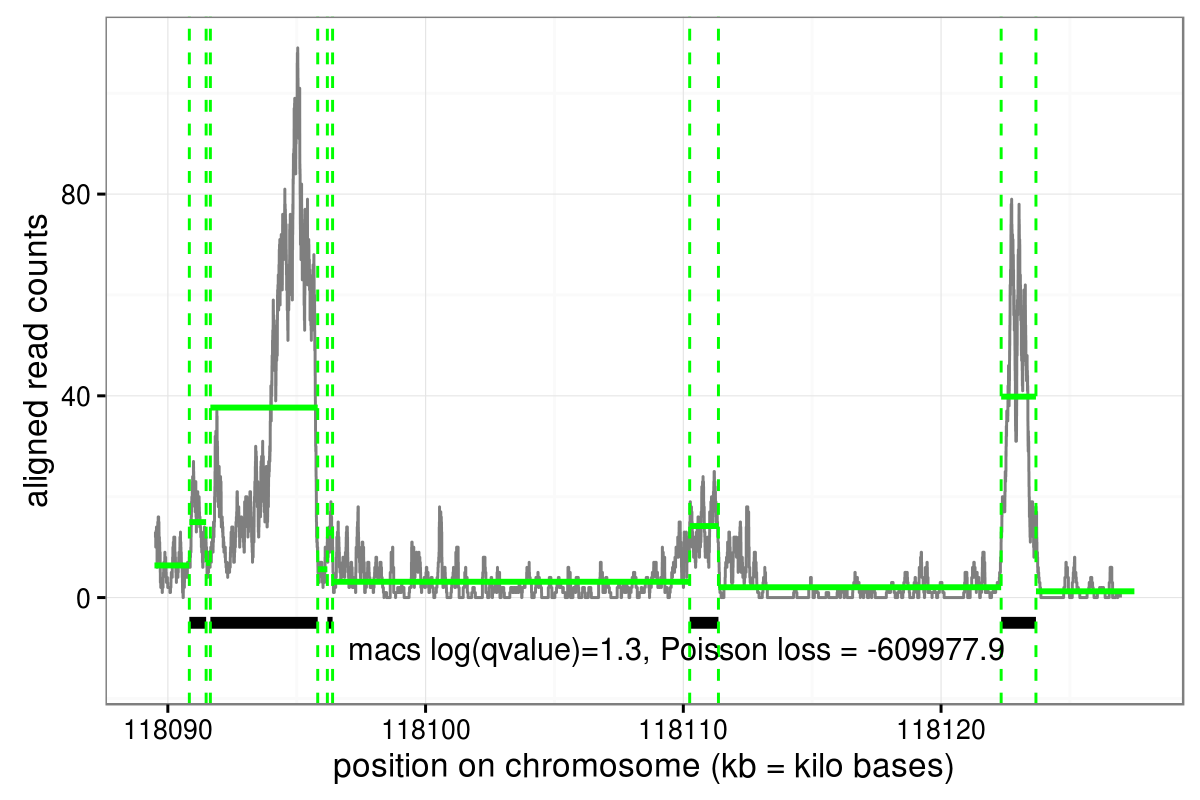
\includegraphics[width=1\textwidth]{figure-macs-problem-1-30103.png}
% \end{frame}

\begin{frame}
  \frametitle{Compute likelihood/loss of piecewise constant model}
  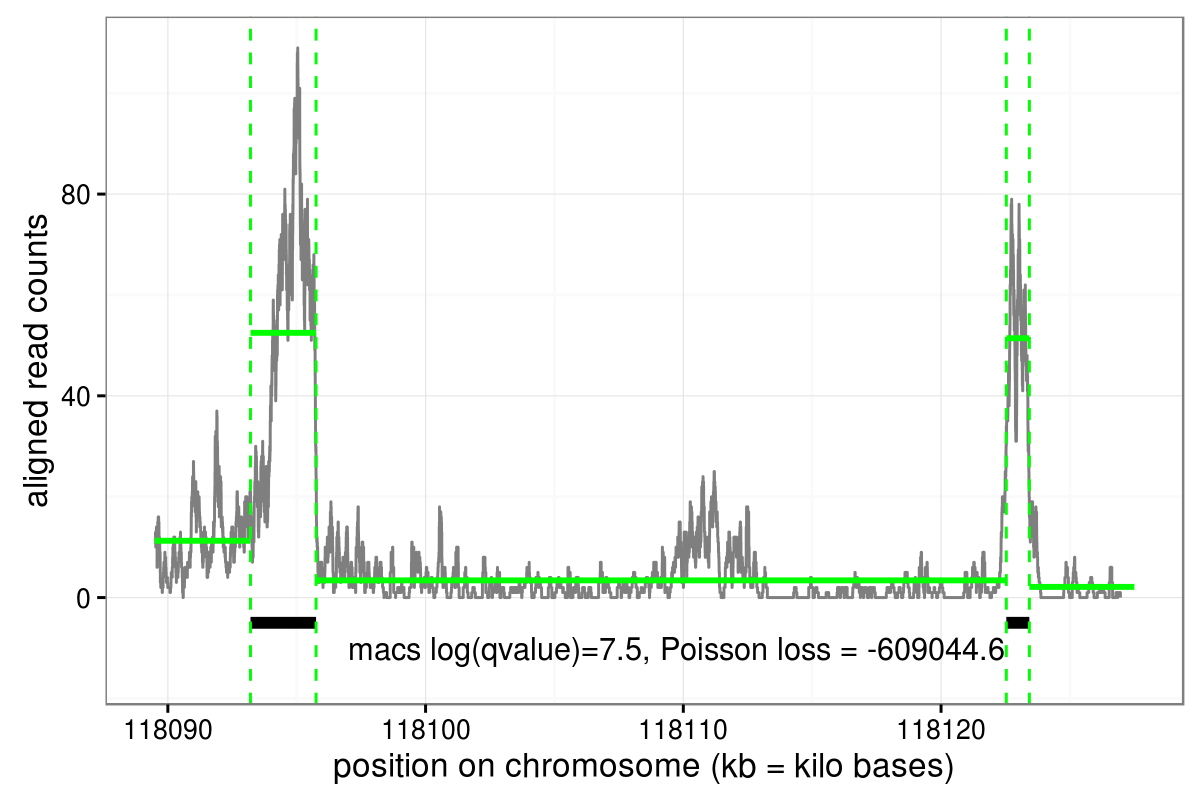
\includegraphics[width=1\textwidth]{figure-macs-problem-7-5.png}
  % $\PoissonLoss(\mathbf z, \mathbf m) = \sum_{i=1}^n m_i - z_i \log(m_i)$
  % for count data $\mathbf z\in\ZZ_+^n$ 
  % and segment mean model $\mathbf m\in\RR^n$.
\end{frame}

\begin{frame}
  \frametitle{Idea: choose the parameter with a lower loss}
  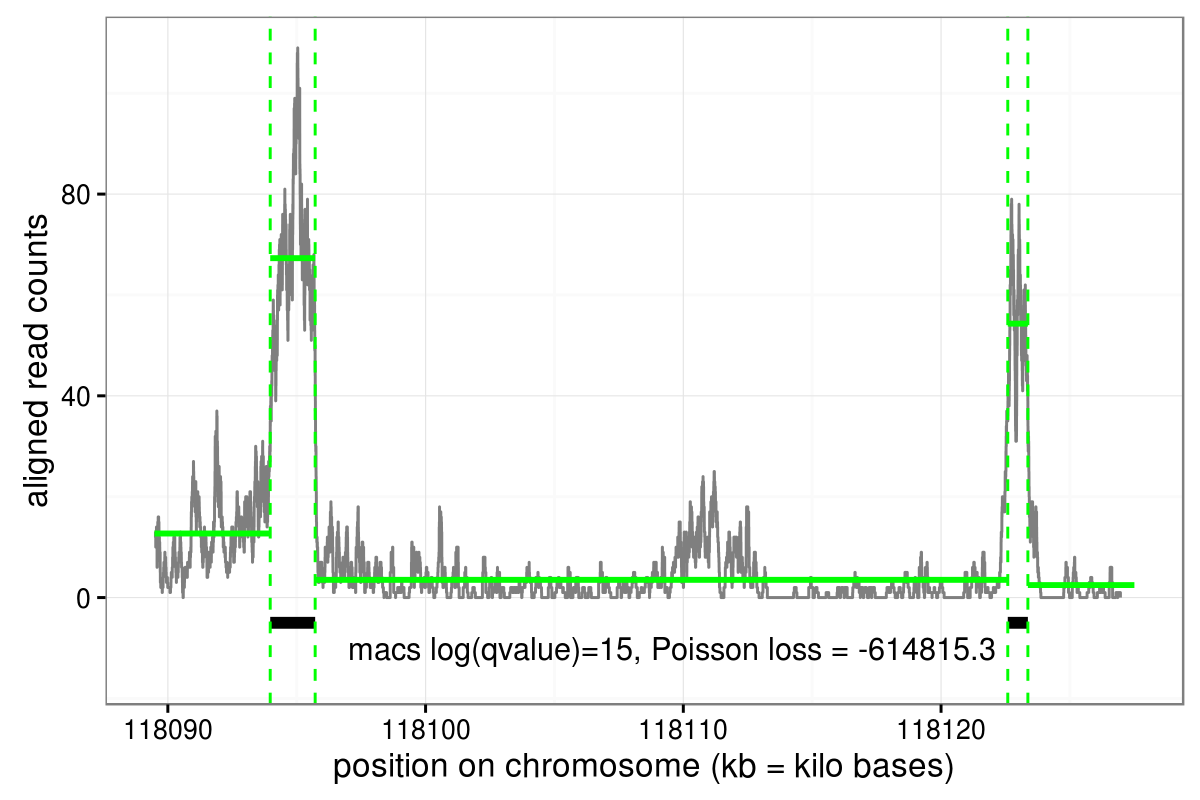
\includegraphics[width=1\textwidth]{figure-macs-problem-15.png}
\end{frame}

\begin{frame}
  \frametitle{PeakSeg: search for the peaks with lowest loss}
  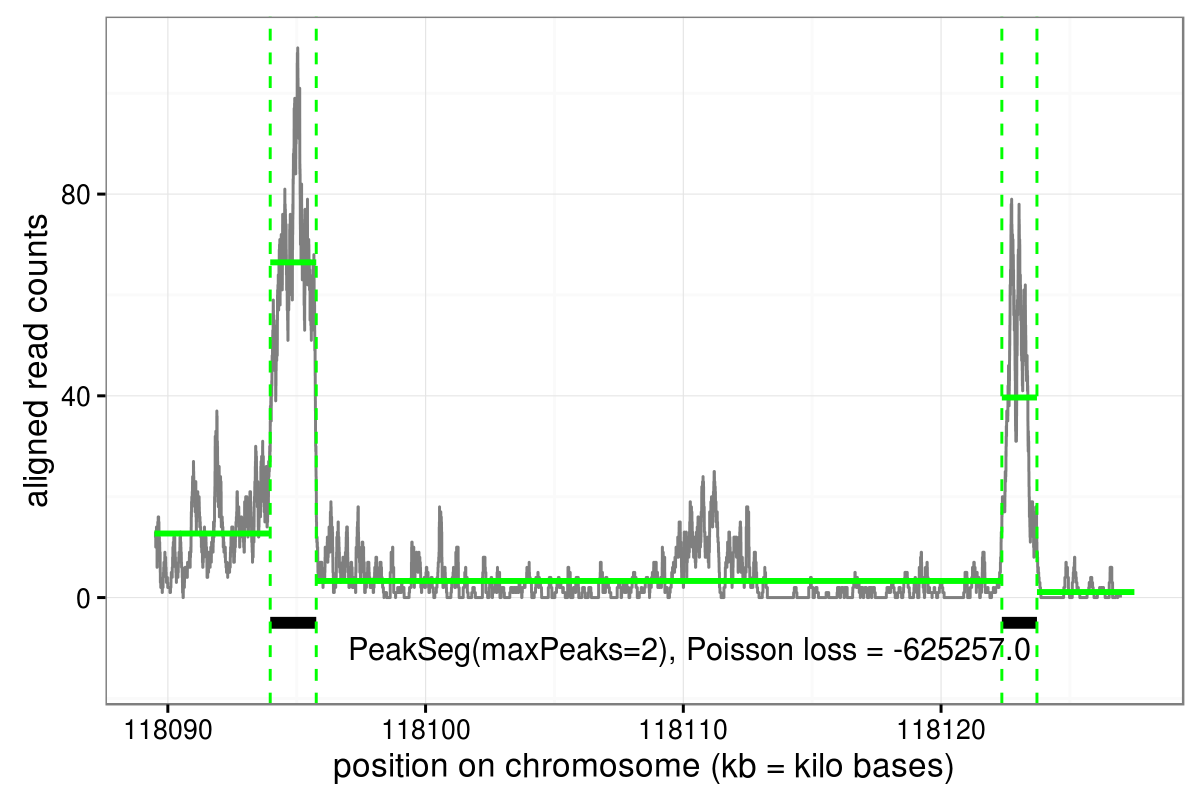
\includegraphics[width=1\textwidth]{figure-macs-problem-PeakSeg.png}
\end{frame}

\section{Algorithm: constrained optimal segmentation}

\begin{frame}
  \frametitle{TODO: PeakSeg undefined slides}
\end{frame}

\begin{frame}
  \frametitle{TODO: unconstrained model not feasible slide}
\end{frame}

\begin{frame}
  \frametitle{TODO: difference with unconstrained PDPA figure
    (min-less function vs min constant)}
\end{frame}

\begin{frame}
  \frametitle{TODO: functional pruning example}
  \url{http://bl.ocks.org/tdhock/raw/8c5dd0af533e24a893e7c5232f9bc94c/}
\end{frame}

\section{Results on benchmark data set}

\begin{frame}
  \frametitle{Linear time algorithm faster for larger data sets}
  \includegraphics[width=1\textwidth]{figure-PDPA-timings.pdf}

  Total time to compute 10 models (0, ..., 9 peaks) for all data sets:
  \begin{itemize}
  \item cDPA: 156 hours, inexact.
  \item cPDPA: 6 hours, exact.
  \end{itemize}
\end{frame}

\begin{frame}
  \frametitle{New coseg algorithm more accurate than unconstrained
    maximum likelihood Poisson model (Segmentor)}
  \includegraphics[width=\textwidth]{figure-min-train-error-Segmentor}
\end{frame}

\begin{frame}
  \frametitle{New coseg algorithm mostly agrees with slower inexact DP}
  \includegraphics[width=\textwidth]{figure-min-train-error-PeakSegDP}
\end{frame}

\begin{frame}
  \frametitle{0 errors for coseg/PeakSegDP, 6 errors for Segmentor}
  \includegraphics[width=\textwidth]{figure-min-train-error-problem2}
\end{frame}

\begin{frame}
  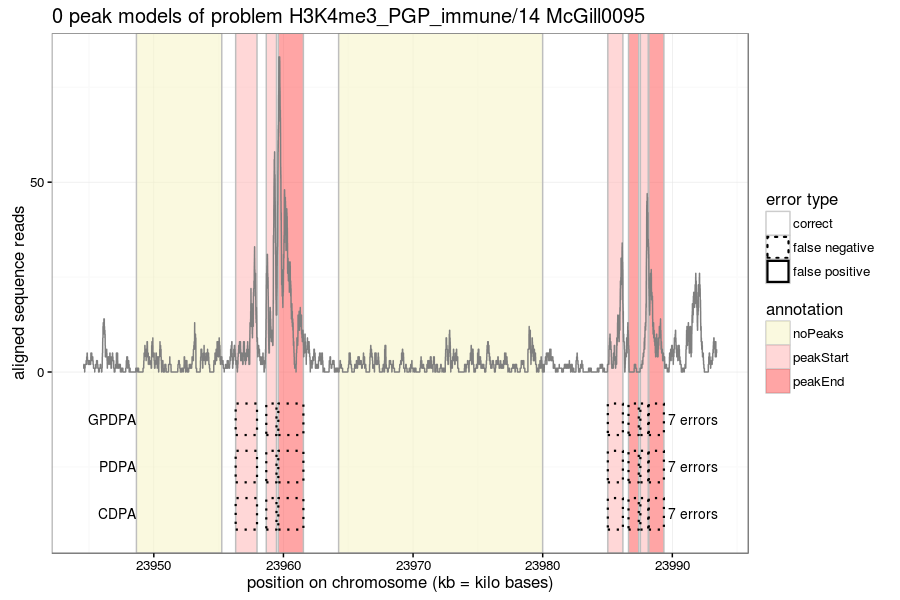
\includegraphics[width=\textwidth]{figure-min-train-error-problem2-0peaks.pdf}
\end{frame}

\begin{frame}
  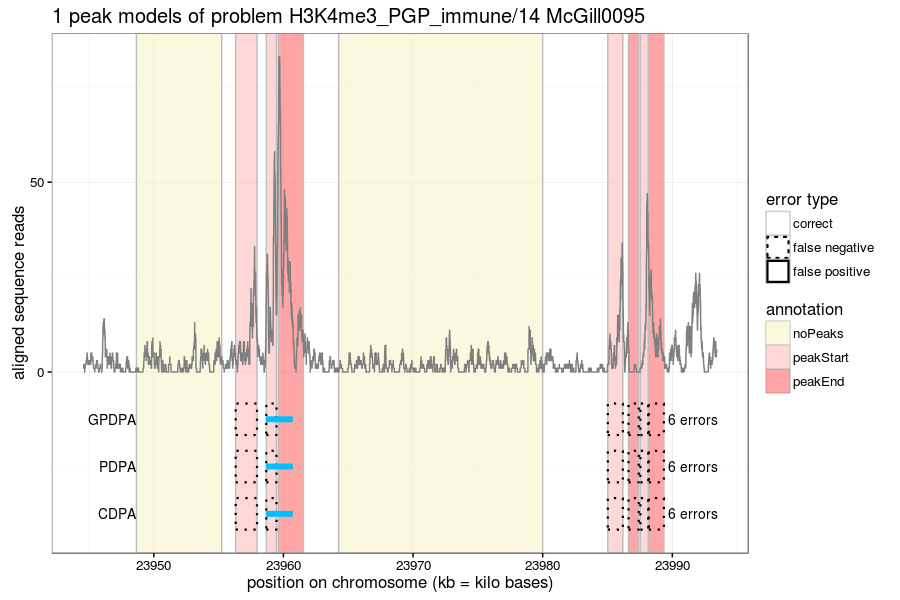
\includegraphics[width=\textwidth]{figure-min-train-error-problem2-1peaks.pdf}
\end{frame}

\begin{frame}
  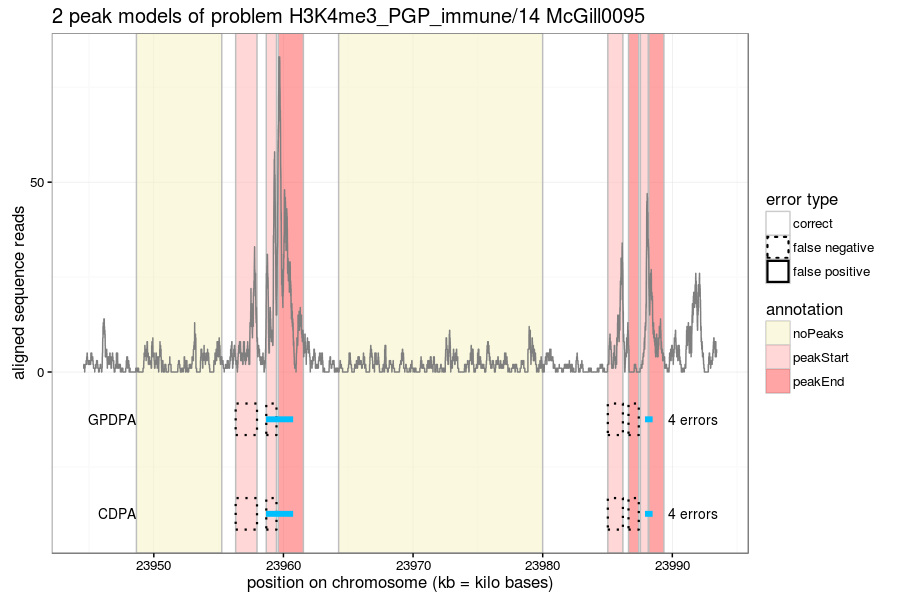
\includegraphics[width=\textwidth]{figure-min-train-error-problem2-2peaks.pdf}
\end{frame}

\begin{frame}
  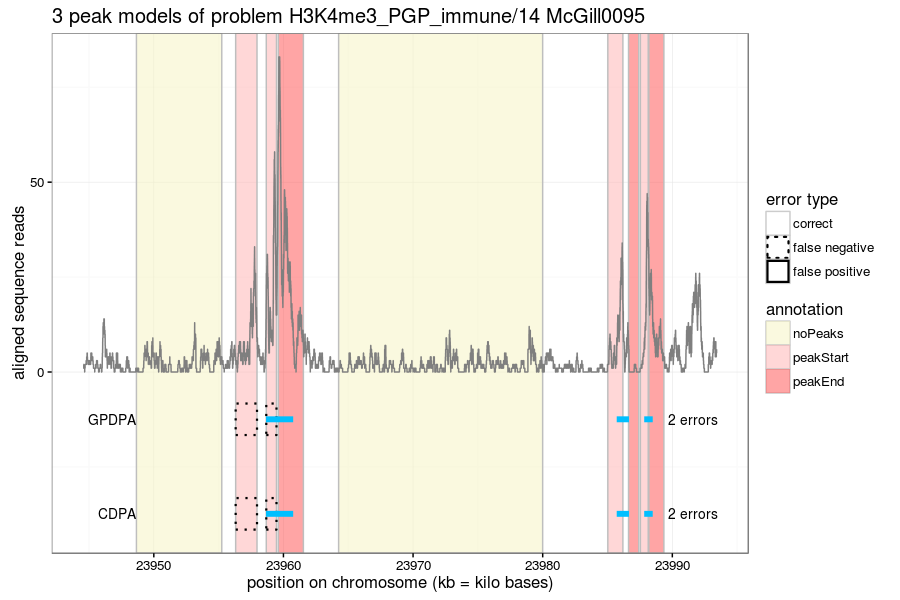
\includegraphics[width=\textwidth]{figure-min-train-error-problem2-3peaks.pdf}
\end{frame}

\begin{frame}
  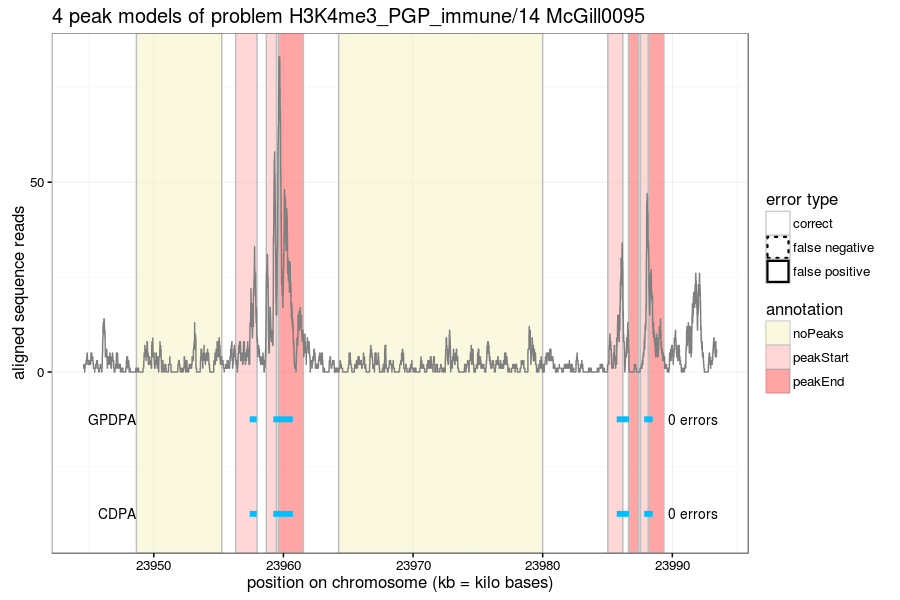
\includegraphics[width=\textwidth]{figure-min-train-error-problem2-4peaks.pdf}
\end{frame}

\begin{frame}
  \frametitle{Errors: PeakSegDP $<$ coseg $<$ Segmentor}
  \includegraphics[width=\textwidth]{figure-min-train-error-problem3}
\end{frame}

\begin{frame}
  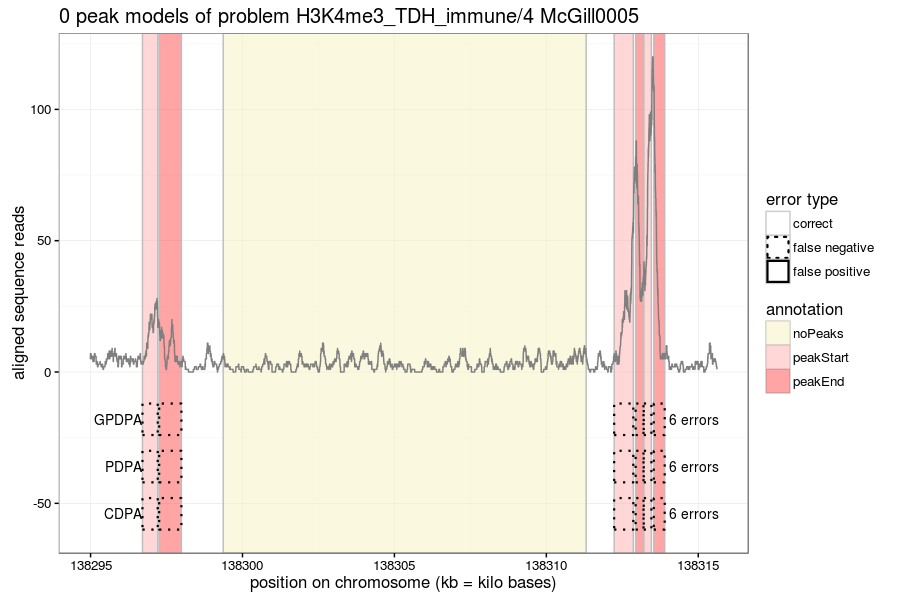
\includegraphics[width=\textwidth]{figure-min-train-error-problem3-0peaks.pdf}
\end{frame}

\begin{frame}
  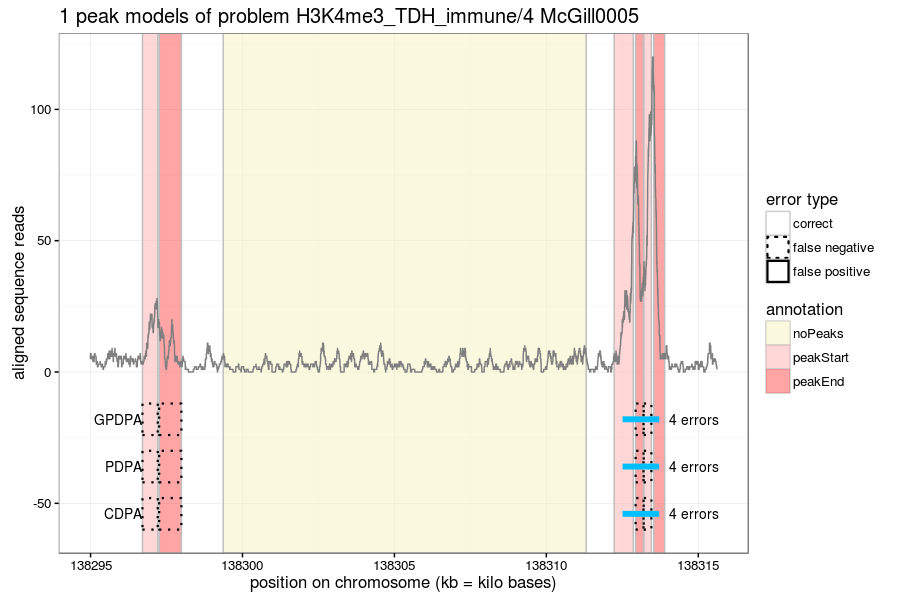
\includegraphics[width=\textwidth]{figure-min-train-error-problem3-1peaks.pdf}
\end{frame}

\begin{frame}
  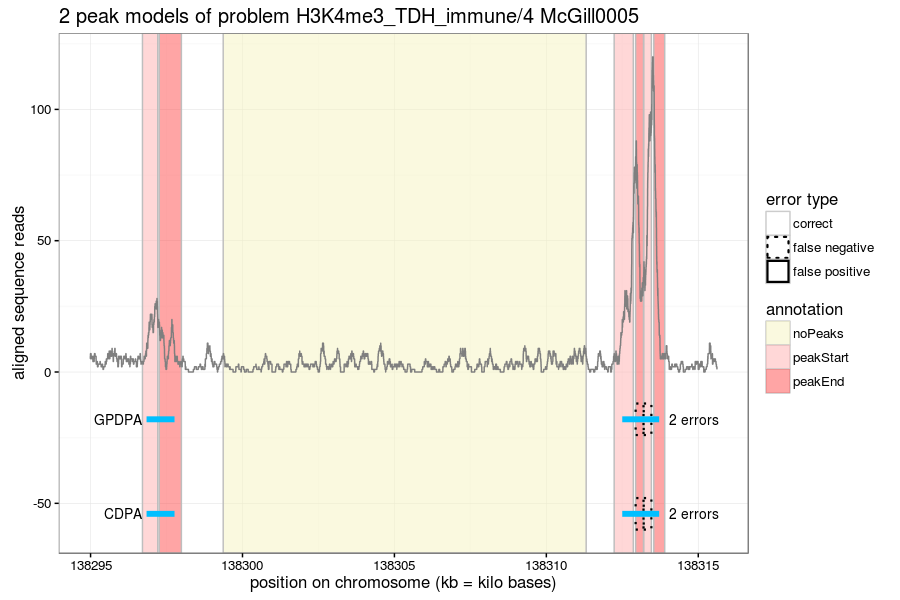
\includegraphics[width=\textwidth]{figure-min-train-error-problem3-2peaks.pdf}
\end{frame}

\begin{frame}
  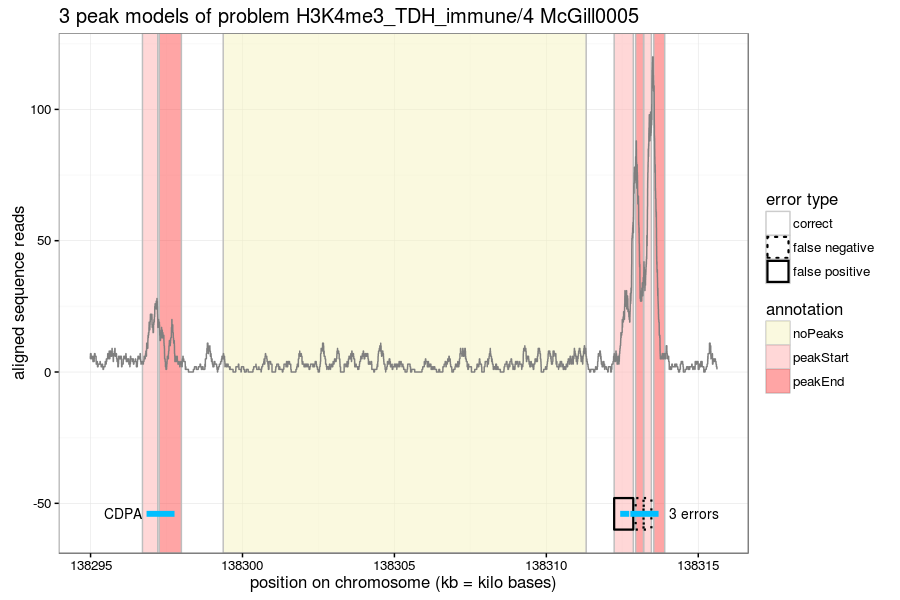
\includegraphics[width=\textwidth]{figure-min-train-error-problem3-3peaks.pdf}
\end{frame}

\begin{frame}
  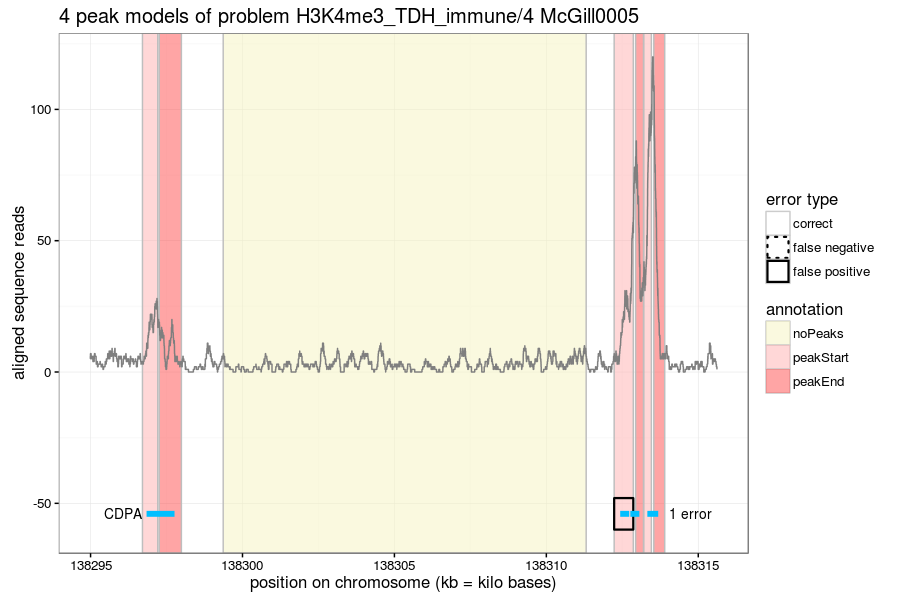
\includegraphics[width=\textwidth]{figure-min-train-error-problem3-4peaks.pdf}
\end{frame}

\begin{frame}
  \frametitle{5 error for coseg/Segmentor, only 1 error for PeakSegDP}
  \includegraphics[width=\textwidth]{figure-min-train-error-problem1}
\end{frame}


\begin{frame}
  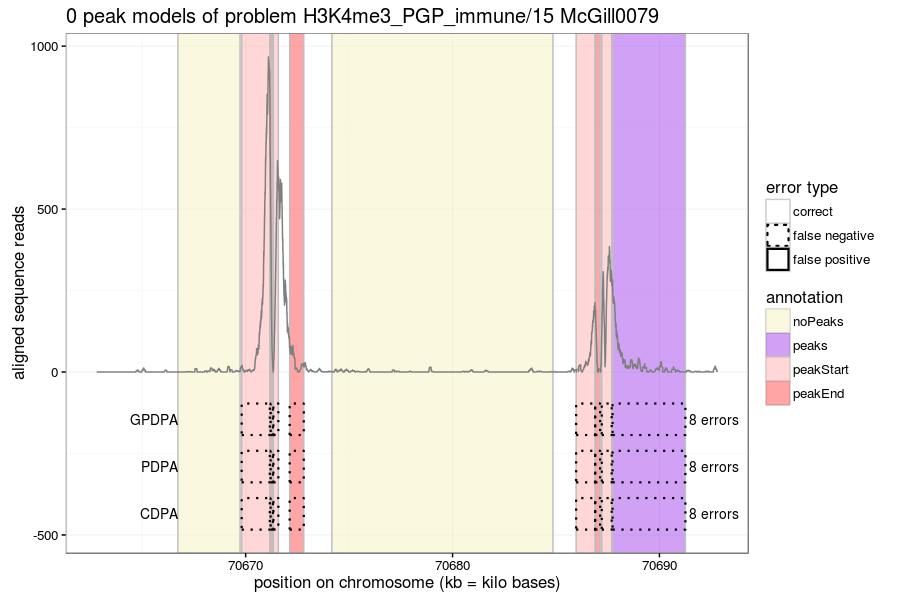
\includegraphics[width=\textwidth]{figure-min-train-error-problem1-0peaks.pdf}
\end{frame}

\begin{frame}
  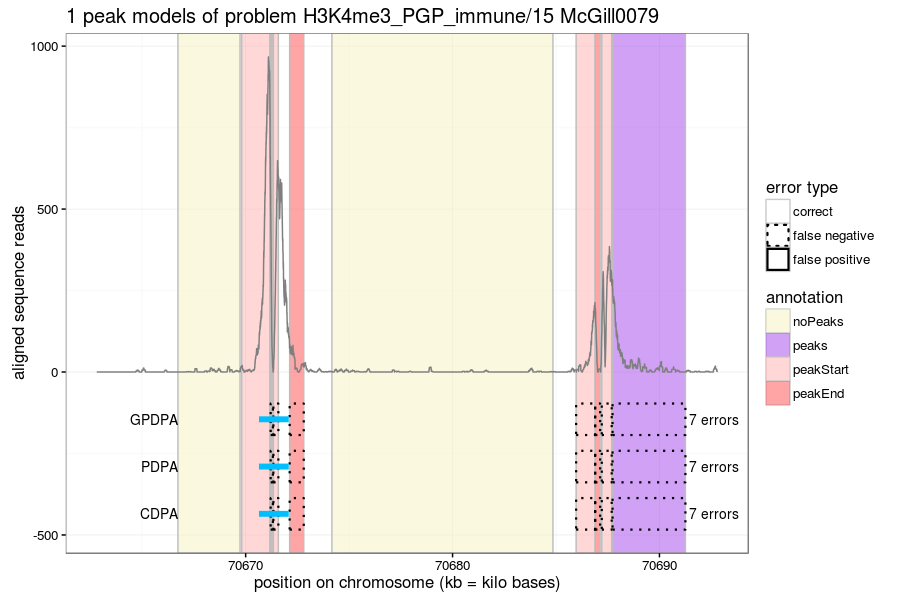
\includegraphics[width=\textwidth]{figure-min-train-error-problem1-1peaks.pdf}
\end{frame}

\begin{frame}
  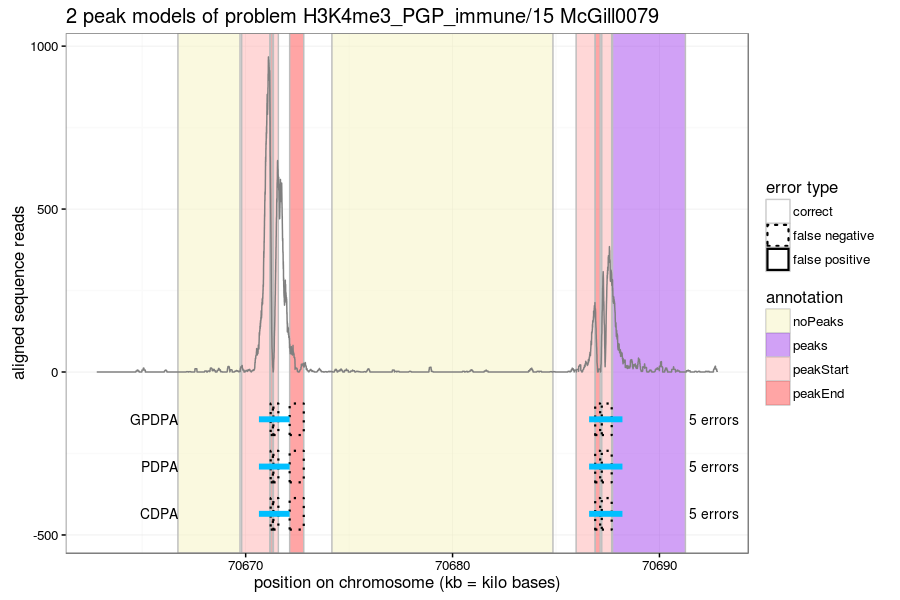
\includegraphics[width=\textwidth]{figure-min-train-error-problem1-2peaks.pdf}
\end{frame}

\begin{frame}
  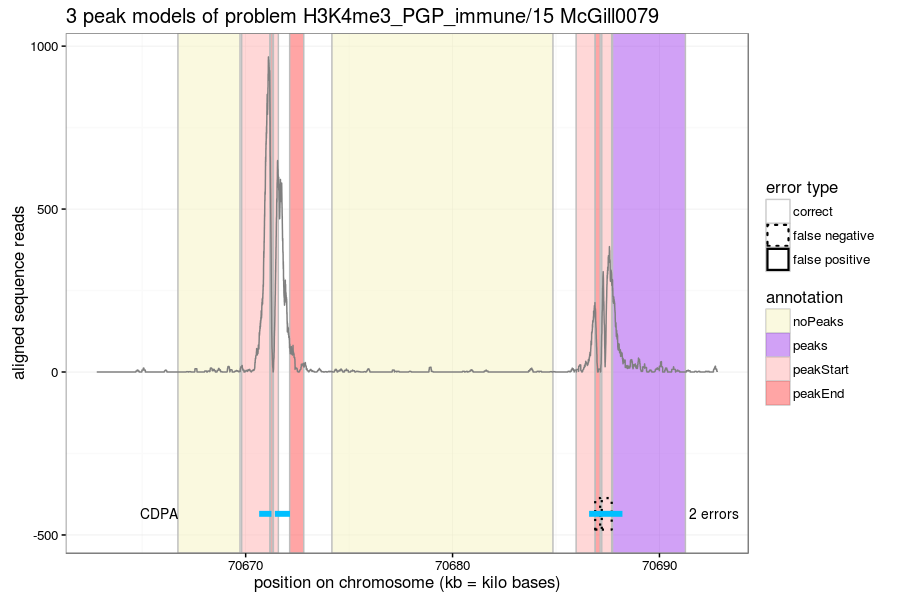
\includegraphics[width=\textwidth]{figure-min-train-error-problem1-3peaks.pdf}
\end{frame}

\begin{frame}
  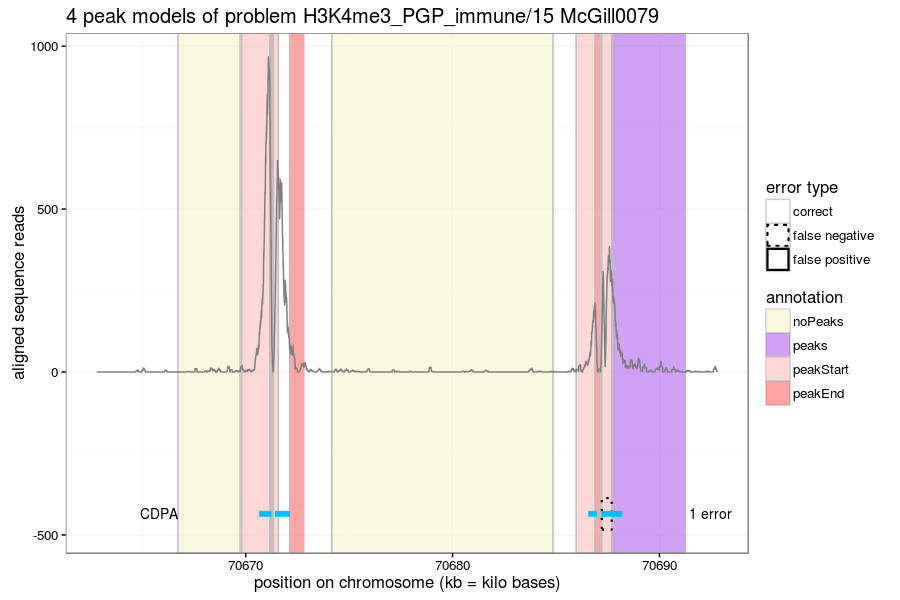
\includegraphics[width=\textwidth]{figure-min-train-error-problem1-4peaks.pdf}
\end{frame}

\section{Future work}

\begin{frame}
  \frametitle{Timings on subsets of human chr1}
  \includegraphics[width=\textwidth]{figure-cosegData-timings-observed.pdf}
\end{frame}

\begin{frame}
  \frametitle{Reasonable predicted time to segment all of chr1}
  \includegraphics[width=\textwidth]{figure-cosegData-timings.pdf}
\end{frame}


\begin{frame}
  \frametitle{Predicted memory requirements too large...}
  \includegraphics[width=\textwidth]{figure-cosegData-timings-memory.pdf}
\end{frame}

\end{document}
